\documentclass[letterpaper,10pt]{article}
\usepackage[margin=0.64in,headheight=12pt,footskip=25pt]{geometry}
\usepackage[T1]{fontenc}
\usepackage{helvet}
\renewcommand{\familydefault}{\sfdefault}
\usepackage{xcolor,graphicx,tabularx,booktabs,enumitem,fancyhdr,hyperref,tikz,tcolorbox}
\usetikzlibrary{arrows.meta,positioning}
\definecolor{Forest}{HTML}{1E4035}
\definecolor{Green}{HTML}{00662C}
\definecolor{Navy}{HTML}{00454D}
\definecolor{Mint}{HTML}{EDF4EF}
\definecolor{Line}{HTML}{C7D8CF}
\definecolor{Ink}{HTML}{18372E}
\definecolor{Muted}{HTML}{4D665B}
\hypersetup{colorlinks=true,linkcolor=Green,urlcolor=Green,pdftitle={PA-40A Participant Guide - TEST ONLY},pdfauthor={ACORN / ORNL}}
\setlength{\parindent}{0pt}
\setlength{\parskip}{6pt}
\setlist[itemize]{topsep=3pt,itemsep=3pt,leftmargin=18pt}
\pagestyle{fancy}\fancyhf{}
\fancyfoot[L]{\color{Muted}\scriptsize PA-40A / TEST ONLY / 11 NOV 2026}
\fancyfoot[R]{\color{Muted}\scriptsize \thepage\ / 5}
\renewcommand{\headrulewidth}{0pt}
\renewcommand{\footrulewidth}{0.4pt}
\newcommand{\eyebrow}[1]{{\color{Green}\small\bfseries #1}\par\vspace{2pt}}
\newcommand{\titleline}[1]{{\color{Forest}\fontsize{22}{26}\selectfont\bfseries #1}\par\vspace{5pt}}
\newcommand{\subline}[1]{{\color{Muted}\small #1}\par\vspace{9pt}}
\newtcolorbox{note}{colback=Mint,colframe=Line,boxrule=.6pt,arc=7pt,left=10pt,right=10pt,top=8pt,bottom=8pt}
\newcommand{\tile}[3]{\node[draw=Line,fill=#3,rounded corners=5pt,minimum width=2.95in,minimum height=.39in,text=Ink,font=\small\bfseries] at (#1) {#2};}
\begin{document}

\eyebrow{PARTICIPANT ORIENTATION}
\titleline{Sponsor Highlights walkthrough}
\subline{A short guide to the published TEST ONLY contributor and reviewer forms. Use invented, non-sensitive content. Work independently and record the first place you hesitate.}

\begin{note}
\textbf{Two roles.} The contributor submits a highlight and checks the receipt and export status. The reviewer opens a Ready batch, inspects a selected item, records a decision, and saves the review. A saved review does not publish a report.
\end{note}

\vspace{12pt}
\eyebrow{ROUTE THROUGH THE TEST WORKFLOW}
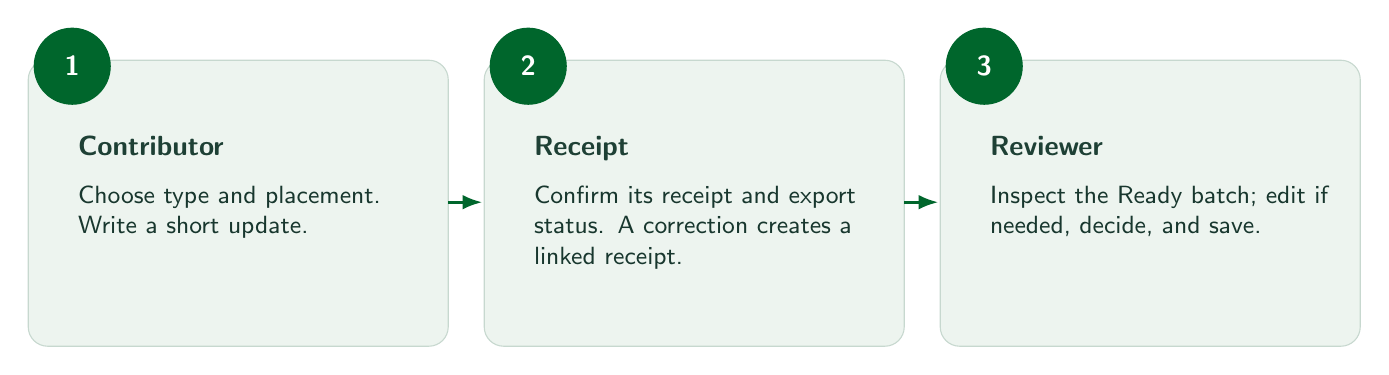
\begin{tikzpicture}[x=1in,y=1in]
  \foreach \x/\number/\heading/\body in {
    0/1/Contributor/{Choose type and placement. Write a short update.},
    2.28/2/Receipt/{Confirm its receipt and export status. A correction creates a linked receipt.},
    4.56/3/Reviewer/{Inspect the Ready batch; edit if needed, decide, and save.}
  }{
    \draw[fill=Mint,draw=Line,rounded corners=7pt] (\x,0) rectangle ++(2.1,1.43);
    \filldraw[fill=Green,draw=Green] (\x+.22,1.40) circle (.19);
    \node[text=white,font=\bfseries] at (\x+.22,1.40) {\number};
    \node[anchor=north west,text=Forest,font=\bfseries] at (\x+.20,1.10) {\heading};
    \node[anchor=north west,text width=1.70in,align=left,font=\small,text=Ink] at (\x+.20,.85) {\body};
  }
  \draw[-{Latex[length=2.5mm]},draw=Green,line width=1pt] (2.10,.72) -- (2.27,.72);
  \draw[-{Latex[length=2.5mm]},draw=Green,line width=1pt] (4.38,.72) -- (4.55,.72);
\end{tikzpicture}

\vspace{16pt}
\eyebrow{BEFORE STARTING}
\begin{enumerate}[leftmargin=20pt,itemsep=6pt]
\item Open the published TEST ONLY app link for your assigned role with your ORNL work account.
\item Confirm the app name. If a connection prompt appears, inspect its services before allowing access.
\item Use fictional people, projects, sponsors, and facts. Do not enter sensitive information.
\item If a task fails, note the exact message and stop that task. Do not repeat a submission or save to work around uncertainty.
\end{enumerate}
\begin{note}
\textbf{What to record:} the first label you could not interpret, a choice you could not find, extra clicks or typing, scrolling that hid the next action, and any failure message. The facilitator should not coach the route before your notes are captured.
\end{note}
\newpage

\eyebrow{CONTRIBUTOR}
\titleline{Submit and correct a highlight}
\subline{Task goal: make one synthetic activity highlight, confirm its receipt, find it in My Submissions, and make one summary correction.}

\begin{tcolorbox}[colback=Forest,colframe=Forest,arc=7pt,left=12pt,right=12pt,top=8pt,bottom=8pt]
{\color{white}\large\bfseries Sponsor Highlights}\hfill {\color{white}\small My Submissions}\par
{\color{white}\small Document progress. Connect research to impact.}
\end{tcolorbox}

\eyebrow{01 / HIGHLIGHT DETAILS}
\begin{tabularx}{\linewidth}{@{}X X@{}}
\textbf{Type} & \textbf{Report placement}\\[4pt]
Activity highlight / Project status & Project highlight / General update\\[12pt]
\textbf{Project} & \textbf{Date}\\[4pt]
Select a project & Choose the activity date\\[12pt]
\textbf{For an activity highlight} & \textbf{For a project status}\\[4pt]
Choose a category, status, and optional event type & Choose project health; choose a risk or None\\
\end{tabularx}

\vspace{10pt}
\eyebrow{02 / THE DEVELOPMENT}
Write the short summary first. Add the context requested for the selected type. Optional details may stay empty. The report preview helps you check how the text reads.

\begin{note}
\textbf{Choice buttons:} project health and risk appear as two-column button grids with icons. A green button and check mark show your selection. All choices in each grid are visible without a separate list scrollbar. For a status marked At risk, Delayed, or Paused, explain the health context. If you choose a risk other than None, add the effect or action needed.
\end{note}

\vspace{8pt}
\eyebrow{FINISH AND CORRECT}
\begin{enumerate}[leftmargin=20pt,itemsep=5pt]
\item Submit once and read the receipt and export status before starting another action.
\item Open My Submissions in the header, select your receipt, then choose Edit selected.
\item Change the summary and save the correction. The original receipt remains; the correction has a linked receipt.
\end{enumerate}

Button icons reinforce the action: arrows move through the form, the circular arrow means refresh or retry, the pencil means edit, and the check means save or selected. Use the text label as the action name.
\newpage

\eyebrow{CONTRIBUTOR REFERENCE VIEWS}
\titleline{Find the status choices}
\subline{The upper image is a historical TEST ONLY reference screenshot. The lower control reference is redrawn from the published November 11 status form because the browser blocked exporting the current capture as a local image. Use the live app for exact placement.}

\begin{center}
\fcolorbox{Line}{white}{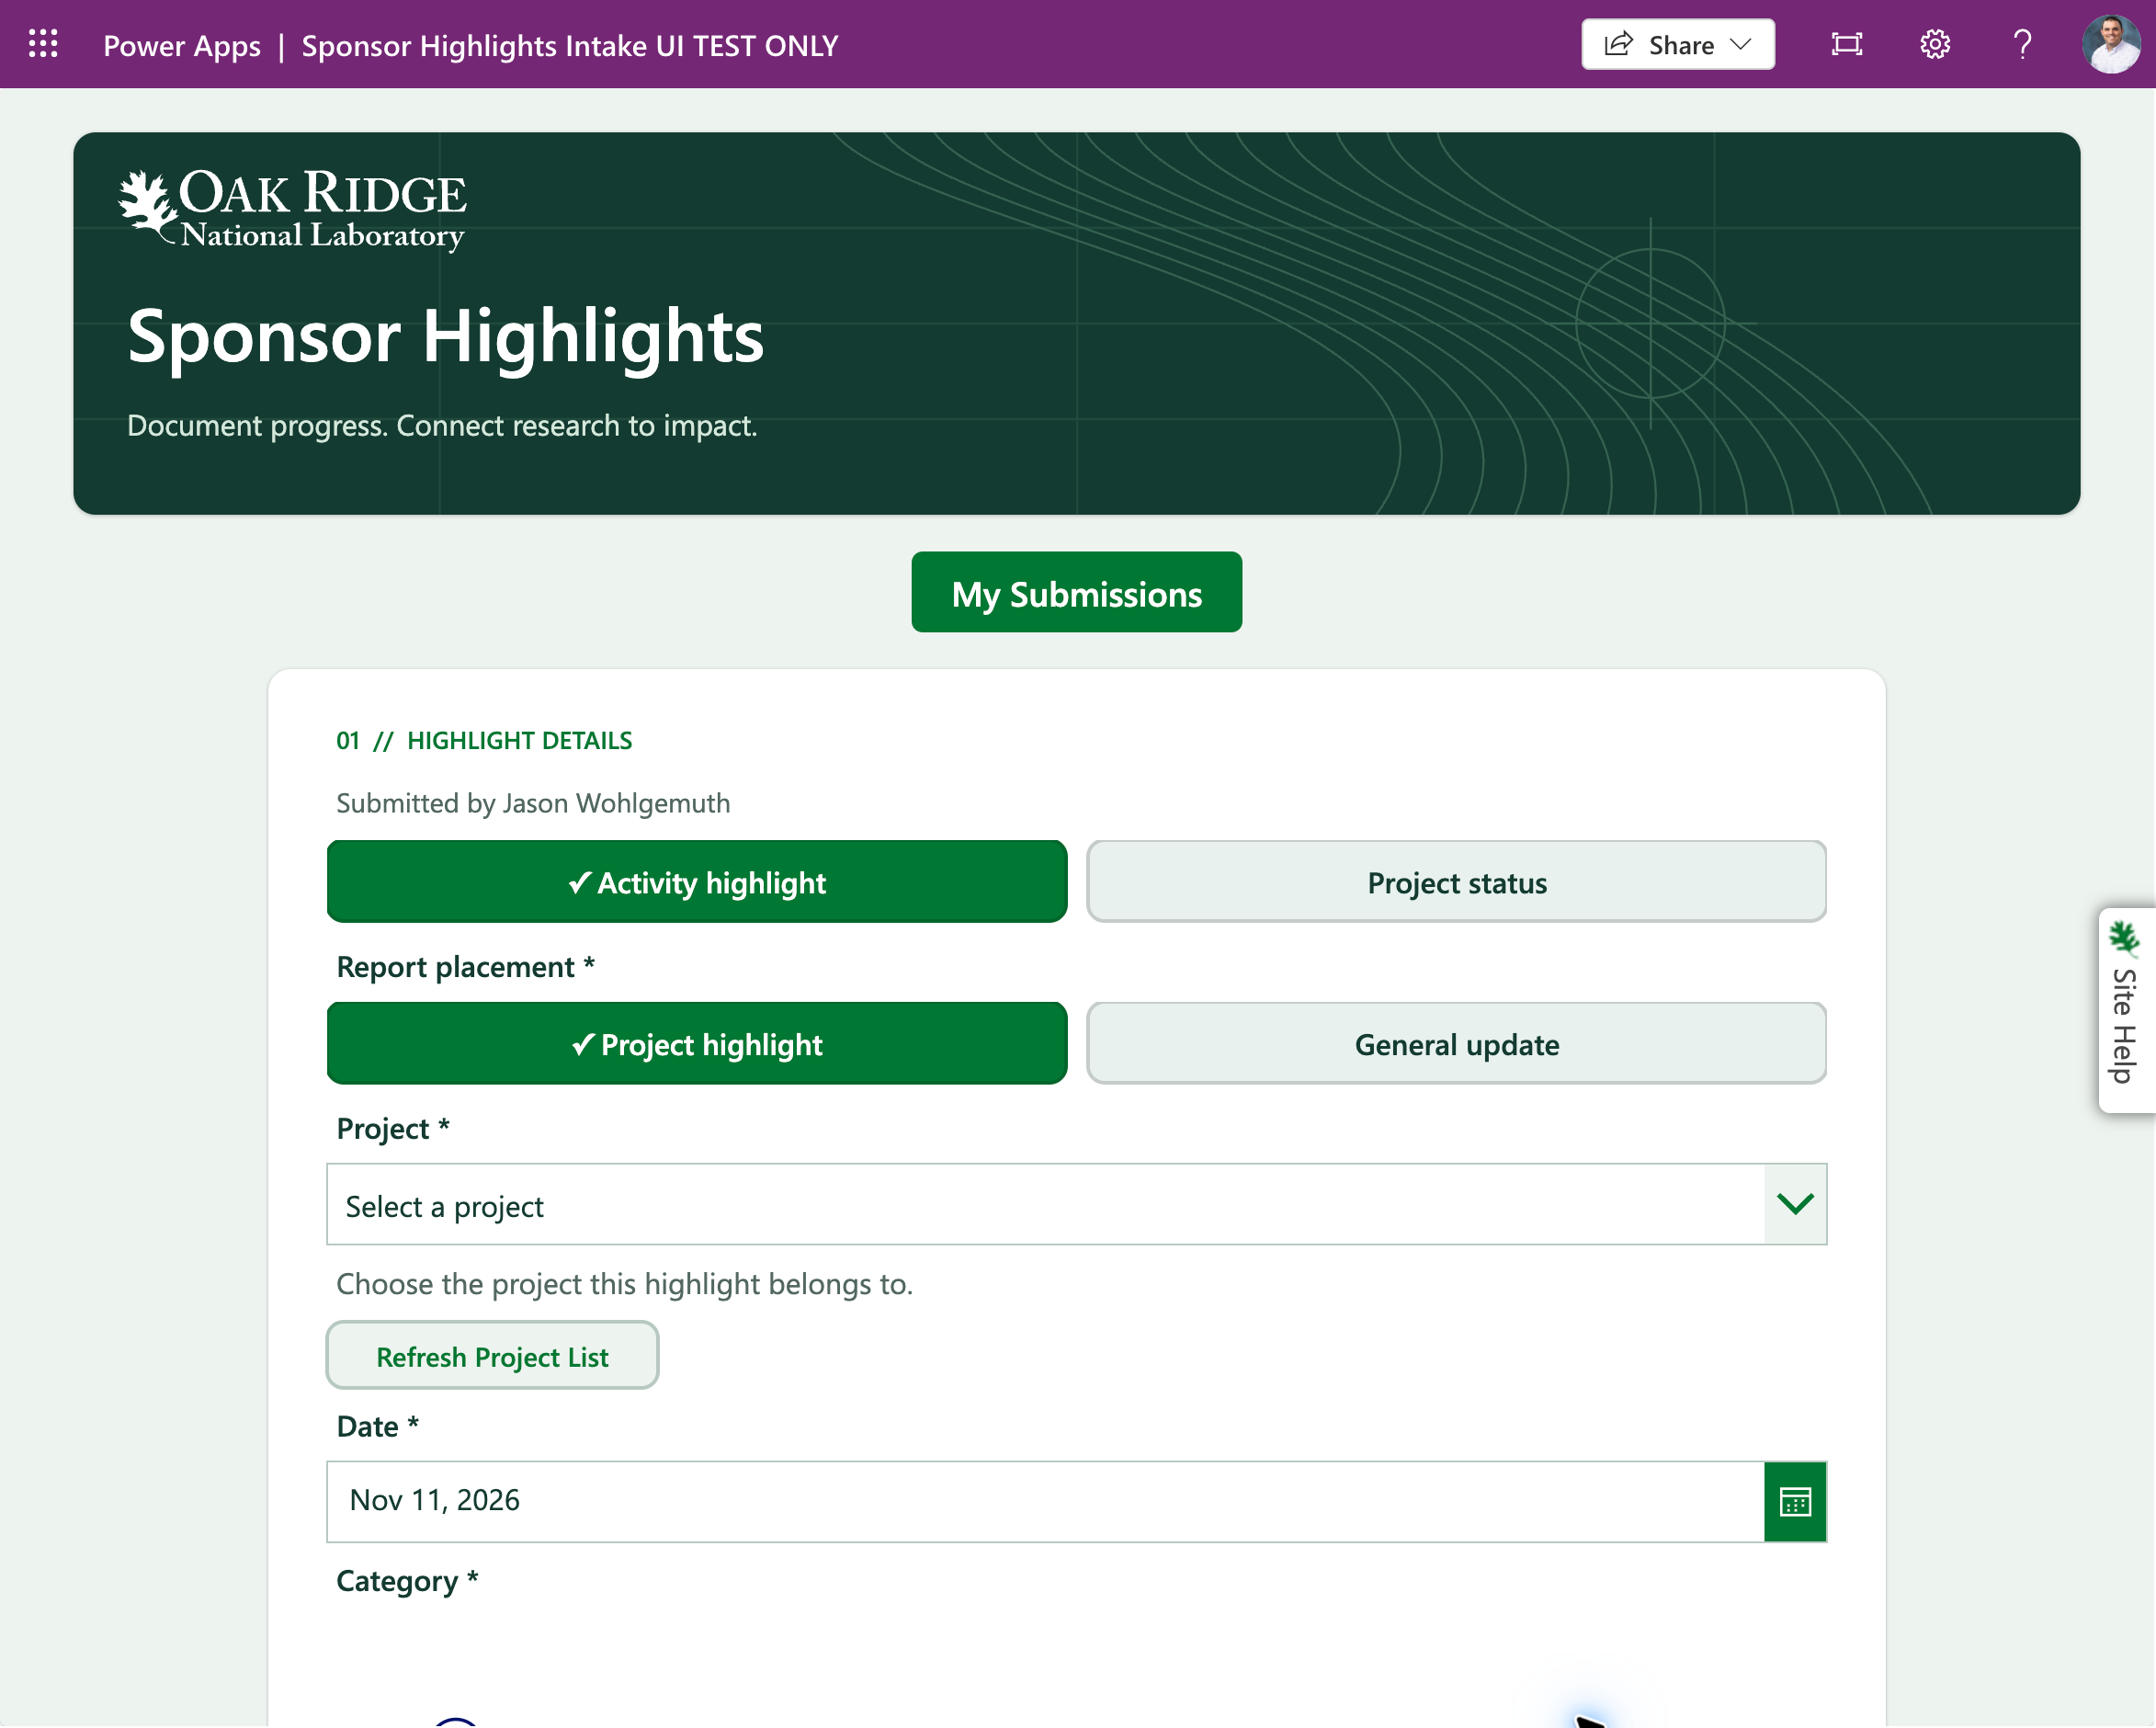
\includegraphics[width=.73\linewidth,height=2.40in,keepaspectratio]{pa40a-contributor-desktop.png}}\\[3pt]
{\color{Muted}\scriptsize Historical reference screenshot: earlier activity form and header.}
\end{center}

\vspace{4pt}
{\color{Forest}\bfseries Current published status controls (redrawn reference)}\par
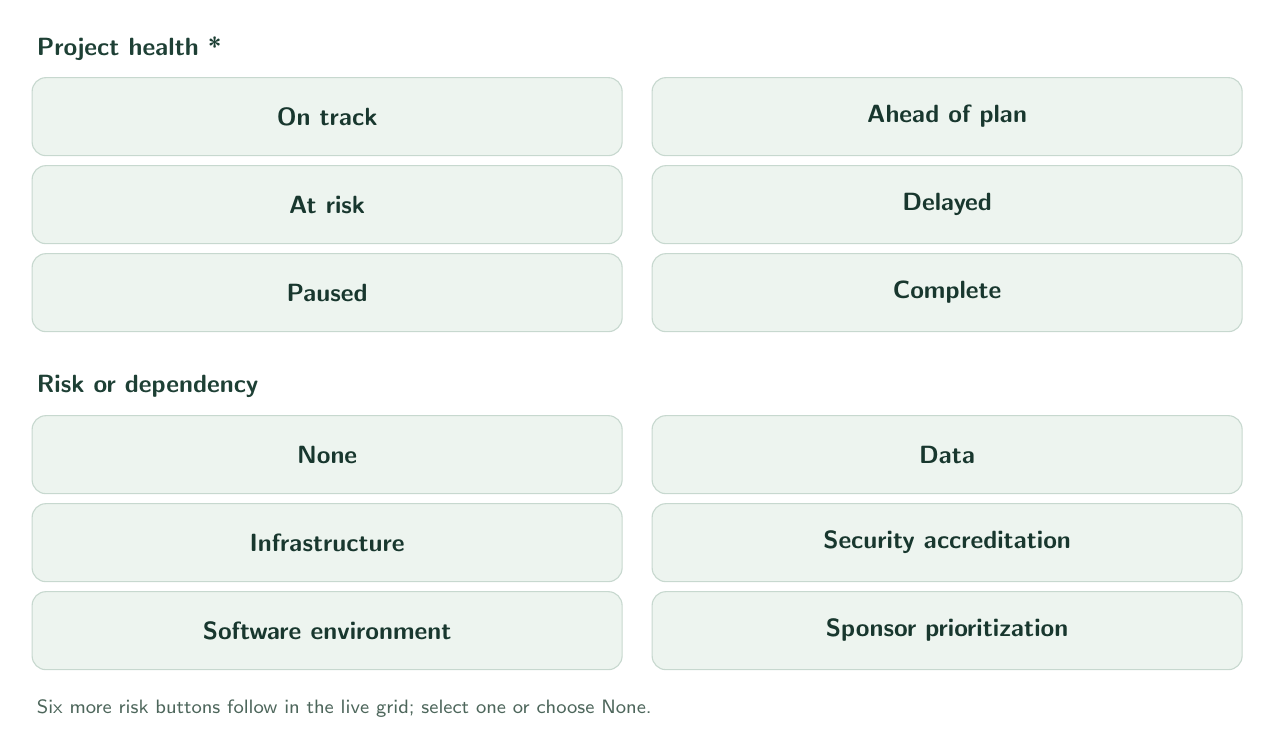
\begin{tikzpicture}[x=1in,y=1in]
  \node[anchor=west,text=Forest,font=\small\bfseries] at (0,0) {Project health *};
  \tile{1.50,-.34}{On track}{Mint}\tile{4.60,-.34}{Ahead of plan}{Mint}
  \tile{1.50,-.78}{At risk}{Mint}\tile{4.60,-.78}{Delayed}{Mint}
  \tile{1.50,-1.22}{Paused}{Mint}\tile{4.60,-1.22}{Complete}{Mint}
  \node[anchor=west,text=Forest,font=\small\bfseries] at (0,-1.69) {Risk or dependency};
  \tile{1.50,-2.03}{None}{Mint}\tile{4.60,-2.03}{Data}{Mint}
  \tile{1.50,-2.47}{Infrastructure}{Mint}\tile{4.60,-2.47}{Security accreditation}{Mint}
  \tile{1.50,-2.91}{Software environment}{Mint}\tile{4.60,-2.91}{Sponsor prioritization}{Mint}
  \node[anchor=west,text=Muted,font=\scriptsize] at (0,-3.30) {Six more risk buttons follow in the live grid; select one or choose None.};
\end{tikzpicture}
\newpage

\eyebrow{REVIEWER}
\titleline{Review a test batch}
\subline{Task goal: load a Ready TEST ONLY batch, inspect one unresolved item, edit its summary if needed, choose a decision, and save. Fixture review is separate local-only practice.}

\begin{tcolorbox}[colback=Forest,colframe=Forest,arc=7pt,left=12pt,right=12pt,top=8pt,bottom=8pt]
{\color{white}\large\bfseries Sponsor Highlights / Review ledger}\hfill{\color{white}\small Load batches}
\end{tcolorbox}

\vspace{5pt}
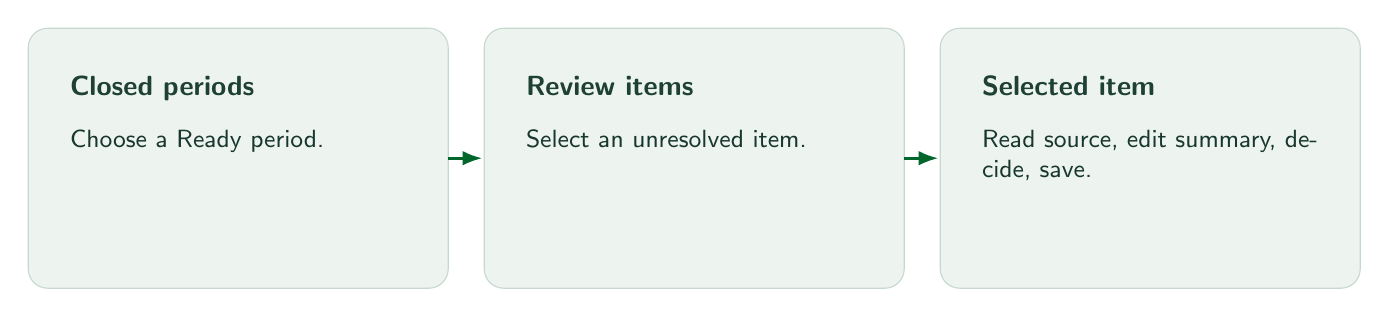
\begin{tikzpicture}[x=1in,y=1in]
  \foreach \x/\head/\body in {
    0/{Closed periods}/{Choose a Ready period.},
    2.28/{Review items}/{Select an unresolved item.},
    4.56/{Selected item}/{Read source, edit summary, decide, save.}
  }{
    \draw[fill=Mint,draw=Line,rounded corners=7pt] (\x,0) rectangle ++(2.1,1.30);
    \node[anchor=north west,text=Forest,font=\bfseries] at (\x+.16,1.11) {\head};
    \node[anchor=north west,text width=1.77in,text=Ink,font=\small] at (\x+.16,.84) {\body};
  }
  \draw[-{Latex[length=2.5mm]},draw=Green,line width=1pt] (2.10,.65) -- (2.27,.65);
  \draw[-{Latex[length=2.5mm]},draw=Green,line width=1pt] (4.38,.65) -- (4.55,.65);
\end{tikzpicture}

\vspace{11pt}
\eyebrow{INSPECT AND DECIDE}
\begin{enumerate}[leftmargin=20pt,itemsep=5pt]
\item Use Needs review to filter the item list. Select an item and read the source summary. View JSON is optional detail.
\item Edit the one summary field if the report text needs work. Choose Unresolved, Approve, or Exclude. Exclude requires a reason.
\item Save the review in the ledger. The optional AI suggestion must be checked against the source before applying it.
\end{enumerate}

\begin{note}
At a narrow browser width, the period, item, and selected-item blocks stack in reading order. The reviewer form uses a short decision row; the fixture practice view uses icon buttons. Saving a review does not publish a report.
\end{note}

\vspace{8pt}
If a Ready batch or item is missing, record that state. Do not save a substitute item to make the walkthrough appear complete.
\newpage

\eyebrow{REVIEWER REFERENCE VIEWS}
\titleline{Find the practice decisions}
\subline{The upper image is a historical TEST ONLY fixture screenshot. The lower decision reference is redrawn from the current published fixture view. The current live ledger is described on page 4.}

\begin{center}
\fcolorbox{Line}{white}{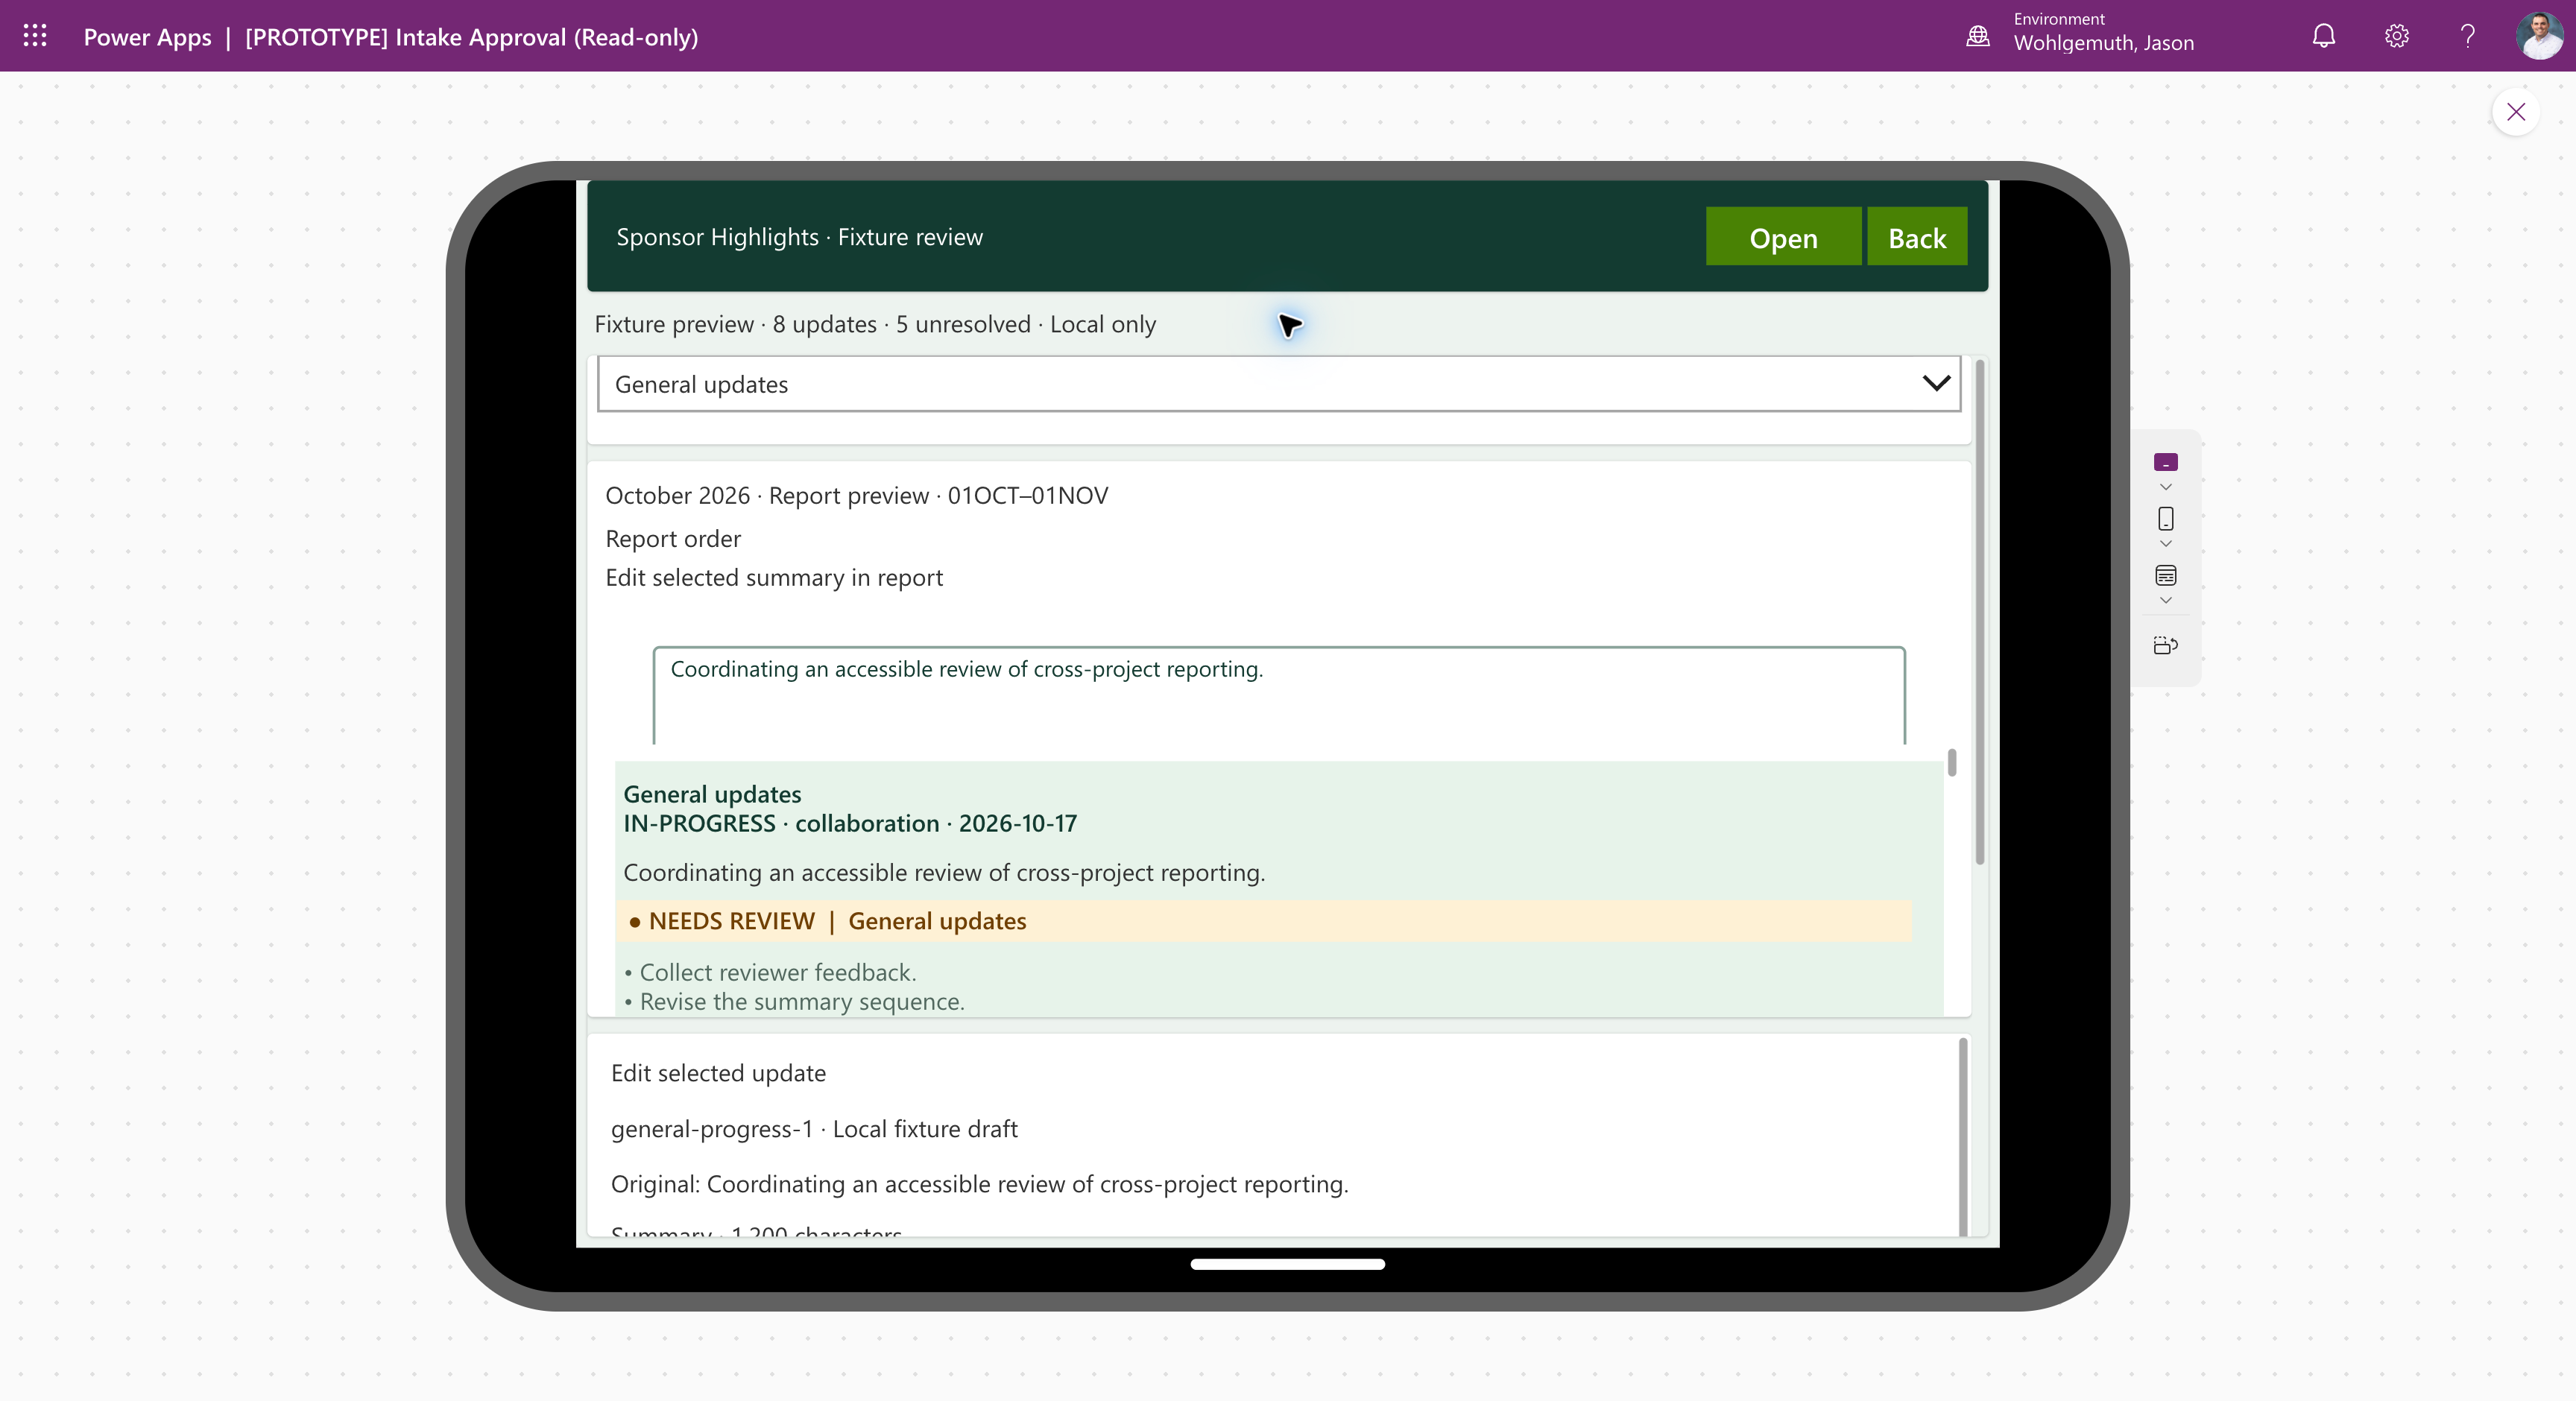
\includegraphics[width=.92\linewidth,height=2.48in,keepaspectratio]{pa40a-reviewer-tablet.png}}\\[3pt]
{\color{Muted}\scriptsize Historical reference screenshot: report preview and inspector.}
\end{center}

\vspace{5pt}
{\color{Forest}\bfseries Current published fixture decision block (redrawn reference)}\par
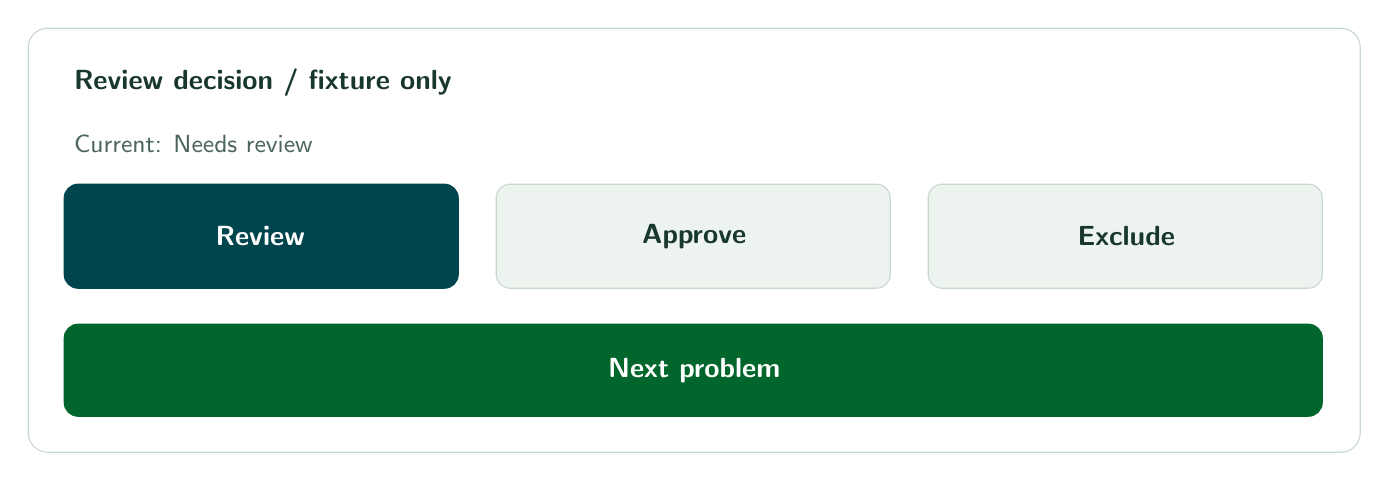
\begin{tikzpicture}[x=1in,y=1in]
  \draw[fill=white,draw=Line,rounded corners=7pt] (0,0) rectangle (6.66,2.12);
  \node[anchor=west,text=Ink,font=\bfseries] at (.18,1.85) {Review decision / fixture only};
  \node[anchor=west,text=Muted,font=\small] at (.18,1.54) {Current: Needs review};
  \draw[fill=Navy,draw=Navy,rounded corners=5pt] (.18,.82) rectangle (2.15,1.34);
  \draw[fill=Mint,draw=Line,rounded corners=5pt] (2.34,.82) rectangle (4.31,1.34);
  \draw[fill=Mint,draw=Line,rounded corners=5pt] (4.50,.82) rectangle (6.47,1.34);
  \node[text=white,font=\bfseries] at (1.16,1.08) {Review};
  \node[text=Ink,font=\bfseries] at (3.33,1.08) {Approve};
  \node[text=Ink,font=\bfseries] at (5.49,1.08) {Exclude};
  \draw[fill=Green,draw=Green,rounded corners=5pt] (.18,.18) rectangle (6.47,.64);
  \node[text=white,font=\bfseries] at (3.33,.41) {Next problem};
\end{tikzpicture}

\begin{note}
\textbf{Record the independent walkthrough:} what you expected, what happened, any label or decision you could not interpret, extra clicks or typing, scrolling that hid the next action, and the exact failure message. Tell the facilitator after you have written the observation.
\end{note}

\end{document}
